%package list
\documentclass{article}
\usepackage[top=3cm, bottom=3cm, outer=3cm, inner=3cm]{geometry}
\usepackage{multicol}
\usepackage{graphicx}
\usepackage{url}
%\usepackage{cite}
\usepackage{hyperref}
\usepackage{array}
%\usepackage{multicol}
\newcolumntype{x}[1]{>{\centering\arraybackslash\hspace{0pt}}p{#1}}
\usepackage{natbib}
\usepackage{pdfpages}
\usepackage{multirow}
\usepackage[normalem]{ulem}
\useunder{\uline}{\ul}{}
\usepackage{svg}
\usepackage{xcolor}
\usepackage{listings}
\lstdefinestyle{ascii-tree}{
    literate={├}{|}1 {─}{--}1 {└}{+}1 
  }
\lstset{basicstyle=\ttfamily,
  showstringspaces=false,
  commentstyle=\color{red},
  keywordstyle=\color{blue}
}
%\usepackage{booktabs}
\usepackage{caption}
\usepackage{subcaption}
\usepackage{float}
\usepackage{array}

\newcolumntype{M}[1]{>{\centering\arraybackslash}m{#1}}
\newcolumntype{N}{@{}m{0pt}@{}}


%%%%%%%%%%%%%%%%%%%%%%%%%%%%%%%%%%%%%%%%%%%%%%%%%%%%%%%%%%%%%%%%%%%%%%%%%%%%
%%%%%%%%%%%%%%%%%%%%%%%%%%%%%%%%%%%%%%%%%%%%%%%%%%%%%%%%%%%%%%%%%%%%%%%%%%%%
\newcommand{\itemEmail}{phidalgo@unsa.edu.pe}
\newcommand{\itemStudent}{Paulo Andre hidalgo Chinchay}
\newcommand{\itemCourse}{Programación web 2}
\newcommand{\itemCourseCode}{20223011}
\newcommand{\itemSemester}{III}
\newcommand{\itemUniversity}{Universidad Nacional de San Agustín de Arequipa}
\newcommand{\itemFaculty}{Facultad de Ingeniería de Producción y Servicios}
\newcommand{\itemDepartment}{Departamento Académico de Ingeniería de Sistemas e Informática}
\newcommand{\itemSchool}{Escuela Profesional de Ingeniería de Sistemas}
\newcommand{\itemAcademic}{2023 - A}
\newcommand{\itemInput}{Del 2 Junio 2023}
\newcommand{\itemOutput}{Al 5 Junio 2023}
\newcommand{\itemPracticeNumber}{01}
\newcommand{\itemTheme}{JavaScript}
%%%%%%%%%%%%%%%%%%%%%%%%%%%%%%%%%%%%%%%%%%%%%%%%%%%%%%%%%%%%%%%%%%%%%%%%%%%%
%%%%%%%%%%%%%%%%%%%%%%%%%%%%%%%%%%%%%%%%%%%%%%%%%%%%%%%%%%%%%%%%%%%%%%%%%%%%

\usepackage[english,spanish]{babel}
\usepackage[utf8]{inputenc}
\AtBeginDocument{\selectlanguage{spanish}}
\renewcommand{\figurename}{Figura}
\renewcommand{\refname}{Referencias}
\renewcommand{\tablename}{Tabla} %esto no funciona cuando se usa babel
\AtBeginDocument{%
	\renewcommand\tablename{Tabla}
}

\usepackage{fancyhdr}
\pagestyle{fancy}
\fancyhf{}
\setlength{\headheight}{30pt}
\renewcommand{\headrulewidth}{1pt}
\renewcommand{\footrulewidth}{1pt}
\fancyhead[L]{\raisebox{-0.2\height}{
\includegraphics[width=3cm]{img/logo_episunsa.png}}}
\fancyhead[C]{\fontsize{7}{7}\selectfont	\itemUniversity \\ \itemFaculty \\ \itemDepartment \\ \itemSchool \\ \textbf{\itemCourse}}
\fancyhead[R]{\raisebox{-0.2\height}{
\includegraphics[width=1.2cm]{img/logo_abet}}}
\fancyfoot[L]{Estudiante Paulo Hidalgo Chinchay}
\fancyfoot[C]{\itemCourse}
\fancyfoot[R]{Página \thepage}

% para el codigo fuente
\usepackage{listings}
\usepackage{color, colortbl}
\definecolor{dkgreen}{rgb}{0,0.6,0}
\definecolor{gray}{rgb}{0.5,0.5,0.5}
\definecolor{mauve}{rgb}{0.58,0,0.82}
\definecolor{codebackground}{rgb}{0.95, 0.95, 0.92}
\definecolor{tablebackground}{rgb}{0.8, 0, 0}

\lstset{frame=tb,
	language=bash,
	aboveskip=3mm,
	belowskip=3mm,
	showstringspaces=false,
	columns=flexible,
	basicstyle={\small\ttfamily},
	numbers=none,
	numberstyle=\tiny\color{gray},
	keywordstyle=\color{blue},
	commentstyle=\color{dkgreen},
	stringstyle=\color{mauve},
	breaklines=true,
	breakatwhitespace=true,
	tabsize=3,
	backgroundcolor= \color{codebackground},
}

\begin{document}
	
	\vspace*{10px}
	
	\begin{center}	
		\fontsize{17}{17} \textbf{ Informe de Laboratorio \itemPracticeNumber}
	\end{center}
	\centerline{\textbf{\Large Tema: \itemTheme}}
	%\vspace*{0.5cm}	

	\begin{flushright}
		\begin{tabular}{|M{2.5cm}|N|}
			\hline 
			\rowcolor{tablebackground}
			\color{white} \textbf{Nota}  \\
			\hline 
			     \\[30pt]
			\hline 			
		\end{tabular}
	\end{flushright}	

	\begin{table}[H]
		\begin{tabular}{|x{4.7cm}|x{4.8cm}|x{4.8cm}|}
			\hline 
			\rowcolor{tablebackground}
			\color{white} \textbf{Estudiante} & \color{white}\textbf{Escuela}  & \color{white}\textbf{Asignatura}   \\
			\hline 
			{\itemStudent \par \itemEmail} & \itemSchool & {\itemCourse \par Semestre: \itemSemester \par Código: \itemCourseCode}     \\
			\hline 			
		\end{tabular}
	\end{table}		
	
	\begin{table}[H]
		\begin{tabular}{|x{4.7cm}|x{4.8cm}|x{4.8cm}|}
			\hline 
			\rowcolor{tablebackground}
			\color{white}\textbf{Laboratorio} & \color{white}\textbf{Tema}  & \color{white}\textbf{Duración}   \\
			\hline 
			\itemPracticeNumber & \itemTheme & 04 horas   \\
			\hline 
		\end{tabular}
	\end{table}
	
	\begin{table}[H]
		\begin{tabular}{|x{4.7cm}|x{4.8cm}|x{4.8cm}|}
			\hline 
			\rowcolor{tablebackground}
			\color{white}\textbf{Semestre académico} & \color{white}\textbf{Fecha de inicio}  & \color{white}\textbf{Fecha de entrega}   \\
			\hline 
			\itemAcademic & \itemInput &  \itemOutput  \\
			\hline 
		\end{tabular}
	\end{table}
	
	\section{Tarea}
	\begin{itemize}		
		\item Utilizando JavaScript, genere un teclado aleatorio para Banca por Internet.
		Funcionalidad: Los números presionados generan una clave.		
		\item Utilizando JavaScript, genere una calculadora como la siguiente imagen. 
		\begin{figure}[H]
			\centering
			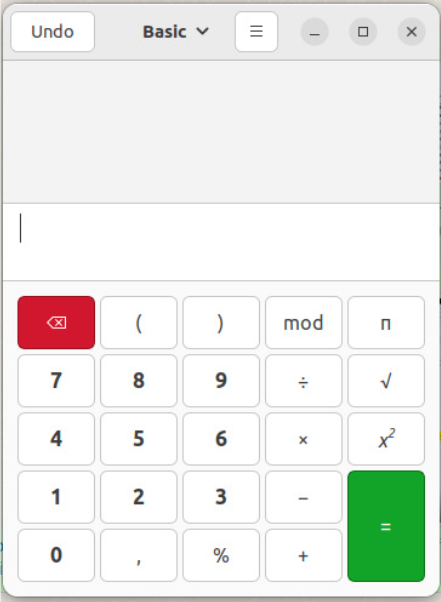
\includegraphics[width=0.3\textwidth,keepaspectratio]{img/calc.png}
		\end{figure}
		Cada vez que se presiona ENTER se guardan los datos involucrados en un pila.		
		Con memoria y botones para recorrer la pila.
		Agregue 4 botones:
		M1: memoria
		M2: memoria
		ANS
	\end{itemize}
		
	\section{Equipos, materiales y temas utilizados}
	\begin{itemize}
		\item Sistema Operativo Ubuntu GNU Linux 23 lunar 64 bits Kernell 6.2.
		\item Sistema Operativo Windows 11 pro versión 22H2 de 64 bits.
		\item VIM 9.0.
		\item Git 2.39.2.
		\item Visual Studio Code 1.78.2.
		\item Cuenta en GitHub con el correo institucional.
		\item Stackoverflow para desordenar un arreglo
		\item \url{https://stackoverflow.com/questions/2450954/how-to-randomize-shuffle-a-javascript-array}
		\item 
	\end{itemize}
	
	\section{URL de Repositorio Github}
	\begin{itemize}
		\item URL del Repositorio GitHub para clonar o recuperar.
		\item \url{https://github.com/PauloUNSA/pw2-lab-c-23a.git}
		\item URL para el laboratorio 01 en el Repositorio GitHub.
		\item \url{https://github.com/PauloUNSA/pw2-lab-c-23a/tree/main/lab1}
	\end{itemize}
	
	\section{Actividades con el repositorio GitHub}
	
	\subsection{Creando e inicializando repositorio GitHub}
	\begin{itemize}	
		\item Como es el primer laboratorio se creo el repositorio GitHub.
		\item Se realizaron los siguientes comandos en la computadora:
		\item Tomando en cuenta que partimos en el directorio HOME \~{}
	\end{itemize}	
		
	\begin{lstlisting}[language=bash,caption={Creando directorio de trabajo}][H]
		$ mkdir -p /paulo/
	\end{lstlisting}
	\begin{lstlisting}[language=bash,caption={Dirijíéndonos al directorio de trabajo}][H]
		$ cd /paulo
	\end{lstlisting}	
	\begin{lstlisting}[language=bash,caption={Creando directorio para repositorio GitHub}][H]
		$ mkdir -p /pw2-lab-c-23a/
	\end{lstlisting}
	\begin{lstlisting}[language=bash,caption={Inicializando directorio para repositorio GitHub}][H]
		$ cd /pw2-lab-c-23a/
		$ vim index.html
		$ git init
		$ git config --global user.name "Paulo Andre Hidalgo Chinchay"
		$ git config --global user.email "phidalgo@unsa.edu.pe"
		$ git add .
		$ git commit -m "paso 1 crear index.html"
		$ git branch -M main
		$ git remote add origin https://github.com/PauloUNSA/pw2-lab-c-23a.git
		$ git push -u origin main
	\end{lstlisting}
	
	\subsection{Commits}
	\begin{lstlisting}[language=bash,caption={Primer Commit Creando archivo index.html para laboratorio 01}][H]
		$ vim index.html
		$ git add .
		$ git commit -m "paso 1 crear index.html"			
		$ git push
	\end{lstlisting}
	\begin{itemize}	
		\item Para el siguiente commit se implemento CSS a nuestra pagina web quedando de la siguiente forma:
	\end{itemize}
	\begin{figure}[H]
		\centering
		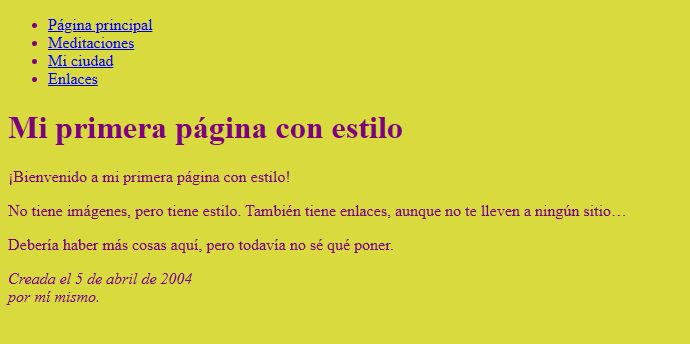
\includegraphics[width=0.8\textwidth,keepaspectratio]{img/Segundo-commit.png}
	\end{figure}
	\begin{itemize}	
		\item El siguiente codigo no incluye ! ni ´ ya que no es reconocido por latex
	\end{itemize}
	\lstinputlisting[language=HTMl, caption={Index.html con CSS},numbers=left,]{src/index01.html}
	
	\begin{itemize}	
		\item Para el ultimo commit se implemento CSS externo a nuestra ya terminada pagina web quedando de la siguiente manera:
	\end{itemize}
	\begin{figure}[H]
		\centering
		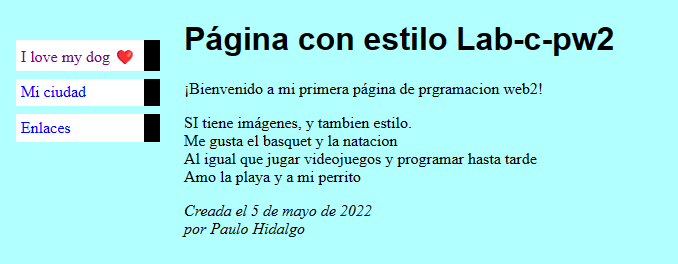
\includegraphics[width=0.8\textwidth,keepaspectratio]{img/ultimo-commit.png}
	\end{figure}

	\begin{itemize}	
		\item Al igual que el anterior código, el no incluye ! ni ´
	\end{itemize}
	\lstinputlisting[language=HTMl, caption={Index.html terminado con CSS externo},numbers=left,]{src/index02.html}
	
	\lstinputlisting[language=HTML, caption={Codigo CSS externo},numbers=left,]{src/css01.css}
	
	\subsection{Estructura de laboratorio 01}
	\begin{itemize}	
		\item El contenido que se entrega en este laboratorio es el siguiente:
	\end{itemize}
	
\begin{lstlisting}[style=ascii-tree]
	C:\USERS\PAULO\PW2-LAB-C-23A\LAB1
	|	estilos.css
	|	index.html
	|---fotos
	|		BusterYYo.jpg
	|---latex
		|	lab1_paulo-hidalgo.tex
		|   lab1_paulo-hidalgo.pdf
		|---build
		|		lab1_paulo-hidalgo.aux
		|       lab1_paulo-hidalgo.fdb_latexmk
		|       lab1_paulo-hidalgo.fls
		|       lab1_paulo-hidalgo.log
		|       lab1_paulo-hidalgo.out
		|       lab1_paulo-hidalgo.pdf
		|       lab1_paulo-hidalgo.synctex.gz
		|---img
		|		logo_abet.png
		|       logo_episunsa.png
		|       logo_unsa.jpg
		|       Segundo-commit.png
		|       ultimo-commit.png
		|---src
		|		css01.css
		|		index01.html
		|		index02.html
\end{lstlisting}    

	\clearpage
	
	\section{\textcolor{red}{Rúbrica para el contenido del Informe y demostración}}
	\begin{itemize}			
		\item El alumno debe marcar o dejar en blanco en celdas de la columna \textbf{Checklist} si cumplio con el ítem correspondiente.
		\item Si un alumno supera la fecha de entrega,  su calificación será sobre la nota mínima aprobada, siempre y cuando cumpla con todos lo items.
		\item El alumno debe autocalificarse en la columna \textbf{Estudiante} de acuerdo a la siguiente tabla:
	
		\begin{table}[ht]
			\caption{Niveles de desempeño}
			\begin{center}
			\begin{tabular}{ccccc}
    			\hline
    			 & \multicolumn{4}{c}{Nivel}\\
    			\cline{1-5}
    			\textbf{Puntos} & Insatisfactorio 25\%& En Proceso 50\% & Satisfactorio 75\% & Sobresaliente 100\%\\
    			\textbf{2.0}&0.5&1.0&1.5&2.0\\
    			\textbf{4.0}&1.0&2.0&3.0&4.0\\
    		\hline
			\end{tabular}
		\end{center}
	\end{table}	
	
	\end{itemize}
	
	\begin{table}[H]
		\caption{Rúbrica para contenido del Informe y demostración}
		\setlength{\tabcolsep}{0.5em} % for the horizontal padding
		{\renewcommand{\arraystretch}{1.5}% for the vertical padding
		%\begin{center}
		\begin{tabular}{|p{2.7cm}|p{7cm}|x{1.3cm}|p{1.2cm}|p{1.5cm}|p{1.1cm}|}
			\hline
    		\multicolumn{2}{|c|}{Contenido y demostración} & Puntos & Checklist & Estudiante & Profesor\\
			\hline
			\textbf{1. GitHub} & Hay enlace URL activo del directorio para el  laboratorio hacia su repositorio GitHub con código fuente terminado y fácil de revisar. &2 &X &2 & \\ 
			\hline
			\textbf{2. Commits} &  Hay capturas de pantalla de los commits más importantes con sus explicaciones detalladas. (El profesor puede preguntar para refrendar calificación). &4 &X &4 & \\ 
			\hline 
			\textbf{3. Código fuente} &  Hay porciones de código fuente importantes con numeración y explicaciones detalladas de sus funciones. &2 &X &2 & \\ 
			\hline 
			\textbf{4. Ejecución} & Se incluyen ejecuciones/pruebas del código fuente  explicadas gradualmente. &2 &X &2 & \\ 
			\hline			
			\textbf{5. Pregunta} & Se responde con completitud a la pregunta formulada en la tarea.  (El profesor puede preguntar para refrendar calificación).  &2 &X &2 & \\ 
			\hline	
			\textbf{6. Fechas} & Las fechas de modificación del código fuente estan dentro de los plazos de fecha de entrega establecidos. &2 &X &2 & \\ 
			\hline 
			\textbf{7. Ortografía} & El documento no muestra errores ortográficos. &2 &X &2 & \\ 
			\hline 
			\textbf{8. Madurez} & El Informe muestra de manera general una evolución de la madurez del código fuente,  explicaciones puntuales pero precisas y un acabado impecable.   (El profesor puede preguntar para refrendar calificación).  &4 &X &4 & \\ 
			\hline
			\multicolumn{2}{|c|}{\textbf{Total}} &20 & &20 & \\ 
			\hline
		\end{tabular}
		%\end{center}
		%\label{tab:multicol}
		}
	\end{table}
	
\clearpage

\section{Referencias}
\begin{itemize}			
	\item \url{https://www.w3.org/Style/Examples/011/firstcss.es.html}
\end{itemize}				
\end{document}